\chapter{Metrics}

\section{Geometric mean (a digression)}
The geometric mean over values $x_1$, $x_2$, … , $x_N$ computes a mean across $N$ values

\begin{equation*}
  GM = (x_1 \cdot x_2 \cdot … \cdot x_N)^{\frac{1}{N}} = \prod_{i}^{N} x_i^{\frac{1}{N}}
\end{equation*}

GM penalizes more (w.r.t .arithmetic mean) the presence of
low values:

\begin{itemize}
  \item Arithmetic mean (0.1, 0.9, 0.9) = 0.633
  \item Geometric mean (0.1, 0.9, 0.9) = 0.433
\end{itemize}

Computing the product of many values can produce numerical instability.
So we often find, instead:

\begin{equation*}
  GM = \exp(\log(\prod_{i}^{N} x_i)) = \exp(\frac{1}{N} \sum_{i}^{N} \ln(x_i))
\end{equation*}


\section{Perplexity}

Perplexity is a metric that quantifies how uncertain the model is in
predicting the (correct) next word

\begin{itemize}
  \item \textbf{High perplexity}: the model is uncertain about the “correct” next word
  \item \textbf{Low perplexity}: the model is certain about the “correct” next word
\end{itemize}
It is quantified in terms of how large the probability assigned to each
next word of a sentence is.

The number represents the average \footnote{Geometric mean} number of words the model is
indecise over, for a sentence.

\paragraph{Example} The dog chased the ...

Probability distribuAon:

\begin{itemize}
  \item P(cat) = 0.25

  \item P(mouse) = 0.15
  \item P(table) = 0.05

  \item P(chair) = 0.1

  \item P(computer) = 0.05
  \item P(tger) = 0.2
  \item P(crocodile) = 0.1

  \item P(owner) = 0.1

  \item P(the) = 0

\end{itemize}

Correct word: cat: P(cat) = 0.25
Even if the vocabulary has 10
words, It's as if the model was
confused between 4 words
(1/0.25 = 0.25-1), each with
equal probability


\subsection{BLEU - limitations}

BLEU is effective if we need to match exact results.
It attempts to capture sequentiality of words with the introduction of
n-grams of various lengths

Is an old metrichs beacuse in some cases is relevant.

However:

\begin{itemize}
  \item BLEU does not care about the \textbf{semantic} of results. Semantically similar sentences are not accepted as valid
  \item  No considerations about \textbf{fluency}, or \textbf{meaning}. Garbage sentences may get relatively large BLEU scores
  \item  \textbf{Word order} ignored beyond n-grams
\end{itemize}

\section{Other metrics}

\begin{itemize}
  \item \textbf{ROUGE} (Recall-Oriented Understudy for Gisting Evaluation)
  \item \textbf{METEOR} (Metric for Evaluation of Translation with Explicit ORdering)
\end{itemize}

\section{BERT Score}
We will use a BERT or similar model to compute a score.
Given Generated sequence G and Reference sequence R. First of all we use the BERT tokenizer.
Tokenize G and R, get output vectors via BERT (or similar model)

Then \textbf{compare} each generated token against each reference token with a similarity function e.g. cosine similarity.

Get a score (0 $\to$ 1) on how similar the predicted vector is (to the most similar
reference vector)

\begin{equation*}
  \text{Precision} = \frac{1}{|G|}\sum_{i} \max_j \operatorname{sim}(G_i, R_j)
\end{equation*}

\paragraph{BERT score example}

\begin{flushleft}
  \begin{minipage}{0.65\linewidth}
    \begin{itemize}
      \item \textbf{Reference}: the dog chased the cat
      \item \textbf{Predicted}: the dog ran aMer the cat
    \end{itemize}

    Precision: get best match for each row

    \begin{itemize}
      \item The $\to$ 0.9967
      \item Dog $\to$ 0.9968
      \item Ran $\to$ 0.9351
      \item Afer $\to$ 0.8868
      \item The $\to$ 0.9921
      \item Cat $\to$ 0.996
    \end{itemize}

    Precision is $\frac{1}{6}(0.9967 + 0.9968 + 0.9351 + 0.8868 + 0.9921 + 0.996) = 0.96725$


    Recall: Get best match for each column

  \end{minipage}%
  \hfill
  \begin{minipage}{0.3\linewidth}
    \centering
    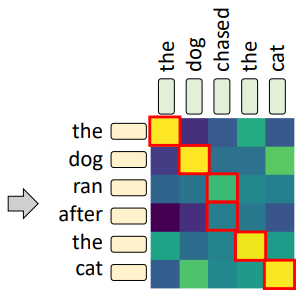
\includegraphics[width=1\linewidth]{content/Parts/images/2026-10-19-10-27-44.png}
  \end{minipage}
\end{flushleft}

BERT score solves the semantica similarity problem. Still does not explicitly consider order. However, tokens are now contextualized, so that helps.

BERT Score relies on an external model. Any limitation of the model reflects on the quality of the result. And, computationally, it is not ideal. Used for simple sentences.

This score does not offer a clear interpretation, "BERT says so".


\section{Exact Match (EM)}

Sometimes, we instead want to match a token/tokens exactly, the output is binary: 1 if is correct, 0 otherwise.



\section{Ranking}

For each token, we can assign a rank to the right word. Ranking the probability distibution the model produces.

\section{Task-specific metrics}

Many tasks are framed so as to get a specific word/words as the
output (fill the blanks).
In that case, classic metrics can be adopted directly.

\section{Human evaluation}

Automated metrics fail to capture concepts like: Coherence, creativity, relevance, fluency
However humans are limited resources:
\begin{itemize}
  \item Costly
  \item Slow process
  \item Evaluation does not scale
\end{itemize}

Common methods:

\begin{itemize}
  \item  Rating scales (e.g., evaluate on a scale from 1 to 5 for fluency)
  \item Pairwise comparisons (e.g., "which of these two sentences is more relevant?")
\end{itemize}

\section{Tasks}

\section{Text completion}
The model is given an incomplete sentence or passage and must
figure out what a plausible continuation is.

The model either generates the correct continuation of the text, or, it chooses the best option among a pool of options.

\subsection{LAMBADA}
A collection of narrative passages. Designed so that humans can guess the word
if they read the entire passage, but not just the last sentence

\subsection{Question Answering (QA)}

There are two type of QA tasks:

\begin{itemize}
  \item \textbf{Open-book QA}: allow the model to “search” the answer in a text/set of texts. Either via Information Retrieval (RAG), or provided via context
  \item \textbf{Closed-book QA}: measure what the model already knows (encoded in its parameters)
\end{itemize}

\section{Translation, summarization}

\begin{itemize}
  \item \textbf{Translation}: Generate the translation of a sentence, and evaluate the quality of the result
  \item \textbf{Summarization}: Generate a summarized version of an original text (e.g., news article). Extractive (select best sentences), or Abstractive (generate new text)
\end{itemize}


\section{Natural Language Inference}

Given a “premise”, NLI is the task to
determine whether a “hypothesis” is:

\begin{itemize}
  \item True (entailment)
  \item False (contradiction)
  \item Undetermined (neutral)
\end{itemize}


\section{Text classification}

Task: classifying sentences into categories based on the contents.

\begin{itemize}
  \item Sentiment analysis
  \item Topic classification
\end{itemize}

\section{Commonsense reasoning}
Commonsense reasoning is the ability to make inferences based on
everyday knowledge of the world:

\begin{itemize}
  \item Cause-effect
  \item Social norms
  \item Reasoning about physical objects
\end{itemize}

Examples of tasks:

\begin{itemize}
  \item ambiguity resolution (infer the intended meaning of words in context)
  \item causal reasoning (infer cause-and-effect relationships)
  \item temporal reasoning (understand sequentiality of events)
  \item physical reasoning (understand the physical domain: permanence, properties, …)
  \item social reasoning (interpret people's/social interactions)
  \item counterfactual reasoning (think about hypothetical scenarios)
\end{itemize}


\section{Benchmarks}
There are various famous benchmarks for LLMs. They cover a wide variety of datasets, and tasks. The purpose is to provide a well-rounded evaluation of models
Leaderboard start here.

\subsection{GLUE}
Used in the early days of LLMs, it contains a set of tasks.
Then superGLUE, but in few years it was outdated.

\subsection{MMLU}
Published in 2020, is a Massive Multitask Language Understanding benchmark, focused on QA with 16K QA with 4 options







